\documentclass[../main.tex]{subfiles}
\begin{document}
\chapter{Integral Theorems}
\section{Green's Theorem in the Plane}
\subsection{Statement and Proof}
\begin{theorem}[Green's Theorem]
  Given an area $A \subset \R^2$ with piecewise smooth boundary $C = \partial A$ and continuously differentiable functions $P(x, y)$ and $Q(x, y)$, then:
  \label{greensTheorem}
  \[
    \int_{A} \left(\pderiv{Q}{x} - \pderiv{P}{y}\right) \d{x} \d{y} = \oint_{C} (P \d{x} + Q \d{y})
  \]
  where $C$ is traversed in the ``positive sense''.

  The ``positive sense'' usually means anti-clockwise, however there are some edge cases involving multiple boundary curves that will be discussed later.
\end{theorem}
\begin{proof}
  Initially, we assume that $A$ is a simple shape.
  This means that for each $y$ there is a single range of values of $x$, namely $x^{-}(y) \leq x \leq x^{+}(y)$.
  Likewise, for each $x$ there is a range $y^{-1}(x) \leq y \leq y^{+}(x)$.
  The diagram below shows an example $y$ and its associated range of values of $x$.
  \begin{center}
  \begin{tikzpicture}[>=stealth]
    \draw[thick, fill=gray!50, postaction={decorate}, decoration={
          markings,
          mark = between positions 0 and 1 step 0.2 with {\arrow{<}}
        }] (-1,1) to[closed, curve through = { (-0.5, 1.3) (0, 1.8) (1, 1.9) (2.5, 0) (1.2, -1.9) (0, -1.6) }] (-1, -1);
    \draw (0, -2) -- (0, 2);
    \draw (-2, 0) -- (3, 0);
    \draw[dotted, thick] (-2, -1.9) -- (3, -1.9) node[right, scale=0.8] {$y_{\text{min}}$};
    \draw[dotted, thick] (-2, 1.97) -- (3, 1.97) node[right, scale=0.8] {$y_{\text{max}}$};
    \filldraw[fill=white, draw=black] (0.55, 1.97) circle (1.5pt) node[above] {$P_1$};
    \filldraw[fill=white, draw=black] (1.1, -1.9) circle (1.5pt) node[below] {$P_2$};
    \node at (2.5, 1.3) {$C^{+}$};
    \node at (-1.3, 1.2) {$C^{-}$};
    \node at (0.6, 0.5) {$A$};

    \draw[dashed] (-0.65, 1.2) -- (2.02, 1.2);
    \fill (0, 1.2) circle (1.5pt) node[below right, scale=0.8] {$y$};
    \draw[dashed] (-0.65, 1.2) -- (-0.65, 0) node[below, scale=0.8] {$x^{-}(y)$};
    \draw[dashed] (2.02, 1.2) -- (2.02, 0) node[below, scale=0.8] {$x^{+}(y)$};
  \end{tikzpicture}
  \end{center}
  We can then divide $C$ into a right hand part $C^{+}$, on which $x = x^{+}(y)$ for each $y$ in the range $y_{\text{min}} \leq y \leq y_{\text{max}}$ and left hand part $C^{-}$ on which $x = x^{-}(y)$.
  In the above diagram, $C^{+}$ goes from $P_2 \to P_1$ and $C^{-}$ goes from $P_1 \to P_2$.

  We can now evaluate the area integral of $\pderiv{Q}{x}$:
  \begin{align*}
    \int_{A} \pderiv{Q}{x} \d{x} \d{y} &= \int_{y_{\text{min}}}^{y_{\text{max}}} \left(\int_{x^{-}(y)}^{x^{+}(y)} \pderiv{Q}{x} \d{x}\right) \d{y} \text{ by definition of area integrals} \\
                                       &= \int_{y_{\text{min}}}^{y_{\text{max}}} [Q(x^{+}(y), y) - Q(x^{-}(y), y)] \d{y} \text{ using FTC} \\
                                       &= \int_{y_{\text{min}}}^{y_{\text{max}}} Q(x^{+}(y), y) \d{y} + \int_{y_{\text{max}}}^{y_{\text{min}}} Q(x^{-}(y), y) \d{y} \\
                                       &= \int_{C^{+}} Q(x, y) \d{y} + \int_{C^{-}} Q(x, y) \d{y} \\
                                       &= \oint Q \d{y}
  \end{align*}
  Similarly, for $\pderiv{P}{y}$:
  \begin{align*}
    \int_{A} \pderiv{P}{y} \d{y} \d{x} &= \int_{x_{\text{min}}}^{x_{\text{max}}} \left(\int_{y^{-}(x)}^{y^{+}(x)} \pderiv{P}{y} \d{y}\right) \d{x} \\
                                       &= \int_{x_{\text{min}}}^{x_{\text{max}}} [P(x, y^{+}(x)) - P(x, y^{-}(x))] \d{x} \text{ using FTC} \\
                                       &= -\int_{x_{\text{max}}}^{x_{\text{min}}} P(x, y^{-}(x)) \d{x} - \int_{x_{\text{min}}}^{x_{\text{max}}} P(x, y^{+}(x)) \d{x} \\
                                       &= -\int_{C^{+}} P(x, y) \d{x} - \int_{C^{-}} P(x, y) \d{x} \\
                                       &= -\oint P \d{x}
  \end{align*}
  So for simple shapes, we are done.

  If $A$ is a more complicated shape (i.e. multiple ranges of $x$ for each $y$ and/or vice versa), then we can split it up into multiple areas $A_i$, each of which is a simple shape, and apply the calculation above to each part to obtain the same result.
  The details of this will be explained below.
\end{proof}
\begin{remark}[Result for non-simple shapes]
  \nonexaminable
  If we have split $A_i$ into disjoint areas then:
  \[
    \int_{A} \pderiv{Q}{x} \d{x} \d{y} = \sum_{i} \int_{A_i} \pderiv{Q}{x} \d{x} \d{y}
  \]
  Furthermore:
  \[
    \oint_{\partial A} Q \d{y} = \sum_{i} \oint_{\partial A_i} Q \d{y}
  \]
  Although each $\partial A_i$ contains a segment not part of the full $\partial A$, these parts cancel out as we have the same segment traversed in different directions in different parts of the shape.

  For example, the following shape has been split into two simple shapes that are infinitesimally close:
  \begin{center}
  \begin{tikzpicture}[>=stealth]
    \draw[thick, fill=gray!50, postaction={decorate}, decoration={
          markings,
          mark = between positions 0.2 and 0.8 step 0.2 with {\arrow{<}}
        }] (0.1, -0.1) to[curve through = { (-0.2, -0.5) (-1, -1) (-1.5, 0) (-0.5, 1.3) (0, 1.8) }] (0.5, 1.9);
    \draw[thick, postaction={decorate}, decoration={
          markings,
          mark = between positions 0.2 and 0.8 step 0.3 with {\arrow{>}}
        }] (0.1, -0.1) -- (0.5, 1.9);

    \begin{scope}[xscale=-1, rotate=23, xshift=-0.4cm, yshift=0.08cm]
      \draw[thick, fill=gray!50, postaction={decorate}, decoration={
            markings,
            mark = between positions 0.2 and 0.8 step 0.2 with {\arrow{>}}
          }] (0.1, -0.1) to[curve through = { (-0.2, -0.5) (-1, -1) (-1.5, 0) (-0.5, 1.3) (0, 1.8) }] (0.5, 1.9);
      \draw[thick, postaction={decorate}, decoration={
            markings,
            mark = between positions 0.2 and 0.8 step 0.3 with {\arrow{<}}
          }] (0.1, -0.1) -- (0.5, 1.9);
    \end{scope}
    \draw (0, -2) -- (0, 2);
    \draw (-2, 0) -- (3, 0);
    \node at (0, 0.9) {$L_1$};
    \node at (-0.9, -0.3) {$A_1$};
    \node at (0.75, 0.8) {$L_2$};
    \node at (0.9, -0.6) {$A_2$};
    \node[scale=0.5] at (0.8, 2.1) {Infinitesimally close};
  \end{tikzpicture}
  \end{center}
  So the sum of the integrals around the boundary of each half is:
  \begin{align*}
    \oint_{\partial A_1} Q \d{y} + \oint_{\partial A_2} Q \d{y} &= \oint_{\partial A} Q \d{y} + \int_{L_1} Q \d{y} + \int_{L_2} Q \d{y} \\
                                                                &= \oint_{\partial A} Q \d{y} + \int_{L_1} Q \d{y} - \int_{L_1} Q \d{y} \\
                                                                &= \oint_{\partial A} Q \d{y}
  \end{align*}
  We can split up $\int_{A} \pderiv{P}{y} \d{x} \d{y}$ using a similar technique and so the result follows for non-simple shapes too.
\end{remark}
\begin{example}[Area of an ellipse]
  Let $A$ be the elliptical region $\frac{x^2}{a^2} + \frac{y^2}{b^2} \leq 1$ and let $P = -\frac{1}{2}y, Q = \frac{1}{2}x$.
  $\pderiv{Q}{x} - \pderiv{P}{y} = 1$ and so:
  \[
    \int_{A} \left(\pderiv{Q}{x} - \pderiv{P}{y}\right) \d{x} \d{y} = \int_{A} 1 \d{x}\d{y} = \text{Area of A}
  \]
  By Greens theorem, this area integral will be the same as the line integral around the boundary ellipse $\partial A$.
  We can parameterise $\partial A$ using $(a \cos t, b \sin t)$, $t \in [0, 2\pi)$ and so:
  \[
    \oint_{\partial A} (P \d{x} + Q \d{y}) = \int_{0}^{2\pi} \left(-\frac{1}{2}b \sin t (-a \sin t) + \frac{1}{2}a \cos t (b \cos t)\right) \d{t} = \pi ab
  \]
  Thus the area of $A$ is $\pi ab$.
\end{example}
\subsection{Multiple Boundary Curves}
Sometimes an area might have two more more boundary curves.
In this case, we can express $A$ as:
\[
  \partial A = \bigcup_{i} C_i
\]
To use Green's theorem here, we have to traverse the outer boundary, say $C_1$, anti-clockwise, but the inner boundaries, say $C_2$ etc, clockwise.
\begin{center}
\begin{tikzpicture}[>=stealth]
  \draw[thick, fill=gray!50, postaction={decorate}, decoration={
        markings,
        mark = between positions 0 and 1 step 0.2 with {\arrow{<}}
      }] (-1,1) to[closed, curve through = { (-0.5, 1.3) (0, 1.8) (1, 1.9) (2.5, 0) (1.2, -1.9) (0, -1.6) }] (-1, -1);

  \draw[thick, fill=white, scale=0.5, postaction={decorate}, decoration={
        markings,
        mark = between positions 0 and 1 step 0.2 with {\arrow{>}}
      }] (-1,1) to[closed, curve through = { (-0.5, 1.3) (0, 1.8) (1, 1.9) (2.5, 0) (1.2, -1.9) (0, -1.6) }] (-1, -1);
  \draw (0, -2) -- (0, 2);
  \draw (-2, 0) -- (3, 0);

  \node at (2, 1.8) {$C_1$};
  \node at (0.5, 0.5) {$C_2$};
  \node at (1.5, 1) {$A$};

  \begin{scope}[xshift=6cm]
    \draw[thick, fill=gray!50, postaction={decorate}, decoration={
          markings,
          mark = between positions 0 and 1 step 0.2 with {\arrow{<}}
        }] (-1,1) to[closed, curve through = { (-0.5, 1.3) (0, 1.8) (1, 1.9) (2.5, 0) (1.2, -1.9) (0, -1.6) }] (-1, -1);

    \draw[thick, fill=gray!20, scale=0.5, postaction={decorate}, decoration={
          markings,
          mark = between positions 0 and 1 step 0.2 with {\arrow{<}}
        }] (-1,1) to[closed, curve through = { (-0.5, 1.3) (0, 1.8) (1, 1.9) (2.5, 0) (1.2, -1.9) (0, -1.6) }] (-1, -1);
    \draw (0, -2) -- (0, 2);
    \draw (-2, 0) -- (3, 0);

    \node at (2, 1.8) {$C_1$};
    \node at (0.5, 0.5) {$-C_2$};
    \node at (1.5, 1) {$A$};
    \node at (0.5, -0.3) {$A_2$};
  \end{scope}
\end{tikzpicture}
\end{center}
In the case where $P$ and $Q$ are defined in all of $A_1$, we can split the area integral over $A_1$ up into two areas.
Let $A_2$ be the interior of $C_2$ and let $A_1 = A \cup A_2$.
We can split the integral over $A_1$ up as $\int_{A_1} =  \int_{A} + \int_{A_2}$.
Then, using the standard version of Greens theorem, $\int_{A_1} = \oint_{C_1}$, and, since we must traverse the curve anticlockwise, $\int_{A_2} = \oint_{-C_2}$.
Thus $\int_{A} = \oint_{C_1} - \oint_{-C_2} = \oint_{C_1} + \oint_{C_2}$.

However, this method only works if $P$ and $Q$ are defined in all of $A_1$, whereas we are given only that they are defined in $A$.
It is quite common for integrands to be undefined at certain points so we would still like to be able to apply Green's Theorem in these cases.
In such cases, consider instead the curve $\widetilde{C}$ with cross cuts $L_1$ and $L_2$ that are arbitrarily close to each other:
\begin{center}
\begin{tikzpicture}[>=stealth]
  \draw[thick, fill=gray!50, postaction={decorate}, decoration={
        markings,
        mark = between positions 0 and 1 step 0.2 with {\arrow{<}}
      }] (-1,1) to[closed, curve through = { (-0.5, 1.3) (0, 1.8) (1, 1.9) (2.5, 0) (1.2, -1.9) (0, -1.6) }] (-1, -1);

  \draw[thick, fill=white, scale=0.5, postaction={decorate}, decoration={
        markings,
        mark = between positions 0 and 1 step 0.2 with {\arrow{>}}
      }] (-1,1) to[closed, curve through = { (-0.5, 1.3) (0, 1.8) (1, 1.9) (2.5, 0) (1.2, -1.9) (0, -1.6) }] (-1, -1);

  \node at (2, 1.8) {$\widetilde{C}$};
  \node at (1.5, 1) {$\widetilde{A}$};

  \fill (0, 0) circle (1.5pt) node[above right, scale=0.5] {Singularity};

  \fill[white] (1.1, -0.2) rectangle (2.6, 0.2);
  \draw[thick, postaction={decorate}, decoration={
        markings,
        mark = at position 0.5 with {\arrow{<}}
      }] (1.235, -0.2) -- (2.522, -0.2) node[midway, below] {$L_1$};
  \draw[thick, postaction={decorate}, decoration={
        markings,
        mark = at position 0.5 with {\arrow{>}}
      }] (1.202, 0.2) -- (2.485, 0.2) node[midway, above] {$L_2$};

  \draw (0, -2) -- (0, 2);
  \draw (-2, 0) -- (3, 0);

  \draw[thick, ->] (3.2, 0) -- (4.8, 0) node[midway, above] {Limiting};
  \begin{scope}[xshift=7cm]
    \draw[thick, fill=gray!50, postaction={decorate}, decoration={
          markings,
          mark = between positions 0 and 1 step 0.2 with {\arrow{<}}
        }] (-1,1) to[closed, curve through = { (-0.5, 1.3) (0, 1.8) (1, 1.9) (2.5, 0) (1.2, -1.9) (0, -1.6) }] (-1, -1);

    \draw[thick, fill=white, scale=0.5, postaction={decorate}, decoration={
          markings,
          mark = between positions 0 and 1 step 0.2 with {\arrow{>}}
        }] (-1,1) to[closed, curve through = { (-0.5, 1.3) (0, 1.8) (1, 1.9) (2.5, 0) (1.2, -1.9) (0, -1.6) }] (-1, -1);

    \node at (2, 1.8) {$C_1$};
    \node at (0.5, 0.5) {$C_2$};
    \node at (1.5, 1) {$\approx A$};

    \fill (0, 0) circle (1.5pt) node[above right, scale=0.5] {Singularity};

    \fill[white] (1.1, -0.05) rectangle (2.6, 0.05);
    \draw[thick, postaction={decorate}, decoration={
          markings,
          mark = at position 0.5 with {\arrow{<}}
        }] (1.239, -0.05) -- (2.517, -0.05) node[midway, below] {$L_1$};
    \draw[thick, postaction={decorate}, decoration={
          markings,
          mark = at position 0.5 with {\arrow{>}}
        }] (1.233, 0.05) -- (2.507, 0.05) node[midway, above] {$L_2$};

    \draw (0, -2) -- (0, 2);
    \draw (-2, 0) -- (3, 0);
  \end{scope}
\end{tikzpicture}
\end{center}
This encloses an area $\widetilde{A}$ and since $P$ and $Q$ are defined in all of $\widetilde{A}$, using the standard Green's Theorem $\int_{\widetilde{A}} = \oint_{\widetilde{C}}$.
In the limit as these cross cuts approach each other, $\widetilde{A}$ becomes the whole of $A$ and $\widetilde{C}$ becomes the whole of $C_1$ and $C_2$ since the cross cuts cancel out in the limit as they are integrals over the same path traversed in opposite directions.
\section{Stokes' Theorem}
\subsection{Statement and Proof}
\begin{theorem}[Stokes' Theorem]
  If $\vec{F}(\vec{x})$ is continuously differentiable vector field and $S$ is a piecewise smooth orientable \textbf{open} surface with piecewise smooth boundary curve $C= \partial S$, then:
  \[
    \int_{S} \nabla \times \vec{F} \cdot \d{\vec{S}} = \oint_{C} \vec{F} \cdot \d{\vec{x}}
  \]
  where $C$ is traversed in the ``positive sense'' with regard to the normal on $S$.

  That is, the flux of $\nabla \times \vec{F}$ through $\vec{S}$ is equal to the line integral of $\vec{F}$ over the boundary of $S$, $C = \partial S$.
\end{theorem}
\begin{remark}
  Green's Theorem in the plane (\cref{greensTheorem}) is a special 2D case of Stoke's Theorem.

  Suppose that $S$ is a flat surface in the plane $z = 0$ and that $\vec{F} = (P, Q, 0)$.
  We then see that $\nabla \times \vec{F} = (0, 0, \pderiv{Q}{x} - \pderiv{P}{y})$ and $\d{S} = (0, 0, 1)\d{x}\d{y}$ and so by Stokes' Theorem:
  \[
    \int_{S} \left(\pderiv{Q}{x} - \pderiv{P}{y}\right) \d{x}\d{y} = \int_{S} \begin{pmatrix}
    0 \\
    0 \\
    \pderiv{Q}{x} - \pderiv{P}{y} \\
    \end{pmatrix} \cdot \begin{pmatrix}
    0 \\
    0 \\
    1 \\
    \end{pmatrix} \d{x} \d{y} =
    \oint_{C} \begin{pmatrix}
    P \\
    Q \\
    0 \\
    \end{pmatrix} \cdot \d{\vec{x}} =
    \oint_{C} (P \d{x} + Q \d{y})
  \]
  which is exactly Green's Theorem.
\end{remark}
For Stokes' Theorem, the \textit{positive sense} is defined \textbf{with regard to the normal} because the notion of ``anti-clockwise'' does not make sense for open surfaces which could be viewed from any side.

The precise rule is that if $\vec{t}$ is the tangent vector for the curve $C$ (see \cref{movingTrihedral}) and $\vec{n}$ is the normal to $S$ at the same point, then $\vec{t} \times \vec{n}$ should point away from the surface.
Note $\vec{n}$ is the \textbf{normal to the surface} and not the principal normal of $C$.
Equivalently, if I walk along $C$ with my feet on $C$ and my head in the direction of $\vec{n}$, the surface should stay on my \textbf{left}.
\begin{remark}[Right Hand Rule]
  In practice, we can instead use a simpler \textit{right hand rule}:

  If your thumb points along $\vec{n}$, your curled fingers indicate the direction $C$ should be traversed.
  This is equivalent to anticlockwise if you are looking down $\vec{n}$ towards the surface.
\end{remark}
\begin{proof}[Stokes' Theorem]
\nonexaminable
  We can prove Stokes' Theorem from Green's Theorem (\cref{greensTheorem}).
  We can parameterise $S$ using $(u, v) \in D \subset R^2$, then by the chain rule:
  \[
    \d{\vec{x}} = \pderiv{\vec{x}}{u} \d{u} + \pderiv{\vec{x}}{v} \d{v}
  \]
  and so:
  \[
    \oint_{C} \vec{F} \cdot \d{\vec{x}} = \oint_{\partial D} \vec{F} \cdot \left(\pderiv{\vec{x}}{u} \d{u} + \pderiv{\vec{x}}{v} \d{v}\right)
  \]
  Now let $P(u, v) = \vec{F}(\vec{x}(u, v)) \cdot \pderiv{\vec{x}}{u}$ and $Q(u, v) = \vec{F}(\vec{x}(u, v)) \cdot \pderiv{\vec{x}}{v}$.
  We can now apply Green's theorem in the $(u, v)$-plane to yield:
  \[
    \oint_{\partial D} \vec{F} \cdot \left(\pderiv{\vec{x}}{u} \d{u} + \pderiv{\vec{x}}{v} \d{v}\right) = \int_{D} \left(\pderiv{Q}{u} - \pderiv{P}{v}\right) \d{u} \d{v}
  \]
  We can use suffix notation to show that:
  \begin{align*}
    \nabla \times \vec{F} \cdot \d{S} &= (\nabla \times \vec{F}) \cdot \left(\pderiv{\vec{x}}{u} \times \pderiv{\vec{x}}{v}\right) \\
                                      &= \levi_{i j k} \levi_{i p q} \pderiv{F_k}{x_j} \pderiv{x_p}{u} \pderiv{x_q}{v} \\
                                      &= \pderiv{F_k}{x_j} \pderiv{x_j}{u} \pderiv{x_k}{v} - \pderiv{F_k}{x_j} \pderiv{x_k}{u} \pderiv{x_j}{v}
  \end{align*}
  We can also show using suffix notation and the chain rule that:
  \begin{align*}
    \pderiv{Q}{u} - \pderiv{P}{v} &= \pderiv{}{u}\left(\vec{F} \cdot \pderiv{\vec{x}}{v}\right) - \pderiv{}{v}\left(\vec{F} \cdot \pderiv{\vec{x}}{u}\right) \\
                                  &= \pderiv{}{x_j}\left(F_k \pderiv{x_k}{v}\right) \pderiv{x_j}{u} - \pderiv{}{x_j}\left(F_k \pderiv{x_k}{u}\right)\pderiv{x_j}{v} \\
                                  &= \pderiv{x_k}{v}\pderiv{}{x_j}(F_k) \pderiv{x_j}{u} - \pderiv{x_j}{v}\pderiv{}{x_j}(F_k) \pderiv{x_k}{u} \\
                                  &= \pderiv{F_k}{x_j} \pderiv{x_j}{u} \pderiv{x_k}{v} - \pderiv{F_k}{x_j} \pderiv{x_k}{u} \pderiv{x_j}{v}
  \end{align*}
  Thus:
  \[
    \pderiv{Q}{u} - \pderiv{P}{v} = \nabla \times \vec{F} \cdot \d{\vec{S}}
  \]
  and so the result follows.
\end{proof}
\begin{example}
  Verify Stokes' Theorem for the open surface $S$ given by $z = (x^2 + y^2)^2$, $0 \leq z \leq 1$ and the vector field $\vec{F} = (x^2 y, 0, 0)$.

  \textbf{Flux Integral}\par
  We can use cylindrical polar coordinates, and so $S$ becomes $z = \rho^4$ and:
  \[
    \vec{x} = \begin{pmatrix}
    \rho \cos \phi \\
    \rho \sin \phi \\
    \rho^4 \\
    \end{pmatrix}
  \]
  To figure out what this looks like, since the surface is radially symmetric, consider the curve $z = x^4,\ x \geq 0$ in the $(x, z)$-plane.
  The surface is then just the surface of revolution of this.

  To find the vector surface element, we can use \cref{dSFormula}:
  \[
    \d{\vec{S}} = -\begin{pmatrix}
    \cos \phi \\
    \sin \phi \\
    4 \rho^3 \\
    \end{pmatrix} \times \begin{pmatrix}
    -\rho \sin \phi \\
    \rho \cos \phi \\
    0 \\
    \end{pmatrix} \d{\rho}\d{\phi} = \begin{pmatrix}
    4\rho^4 \cos \phi \\
    4\rho^4 \sin \phi \\
    -\rho \\
    \end{pmatrix} \d{\rho}\d{\phi}
  \]
  where we chose the $-$ sign so we get the downwards-facing normal.
  Note this is not an ``outwards'' facing normal as the surface is open so does not have a notion of being inside or outside.

  Now:
  \[
    \nabla \times \vec{F} = \begin{pmatrix}
    0 \\
    0 \\
    -x^2 \\
    \end{pmatrix} = \begin{pmatrix}
    0 \\
    0 \\
    -\rho^2 \cos^2 \phi \\
    \end{pmatrix}
  \]
  and so:
  \[
    \int_{S} \nabla \times \vec{F} \cdot \d{\vec{S}} = \int_{\rho = 0}^{1} \int_{\phi = 0}^{2\pi} \rho^3 \cos^2 \phi \d{\phi} \d{\rho} = \frac{\pi}{4}
  \]

  \textbf{Boundary Integral}\par
  The boundary $C = \partial S$ is just the curve $x^2 + y^2 = 1,\ z = 1$, or in cylindrical polars $\rho = 1,\ z = 1,\ \phi \in [0, 2\pi)$.
  To figure out which direction we use, the right hand rule tells us that we must traverse $C$ in the direction of decreasing $\phi$.

  We can parameterise $C$ as $x = \cos \phi$, $y = \sin \phi$, $z = 1$ where $\phi$ decreases from $2\pi$ to $0$.
  Therefore, the line integral over $C$ is:
  \[
    \oint_{C} \vec{F} \cdot \d{\vec{x}} = \int_{2\pi}^{0} x^2 y \deriv{x}{\phi} \d{\phi} = - \int_{2\pi}^{0} \cos^2 \phi \sin^2 \phi \d{\phi} = \frac{\pi}{4}
  \]
  So they agree, as expected.
\end{example}
\subsection{Closed Surfaces}
Although we stated that Stoke's Theorem is for open surfaces, it also applies to closed surfaces $S$.
However, for a closed surface $S$, $\partial S = \emptyset$ and so the line integral over $\partial S$ is 0.
This means that:
\[
  \oiint_S \nabla \times \vec{F} \cdot \d{\vec{S}} = 0
\]
\subsection{Multiple Boundary Curves}
Similarly to how in Green's Theorem we have to consider what happens when an area has multiple boundary curves, an open surface may have multiple boundary curves.
We have to apply the right hand rule for the directions of $\vec{n}$ and the direction the curve is traversed separately for each boundary which \textit{usually} results in opposite orientations for each boundary.
\subsection{Extended Example}
\begin{remark}[Question]
  Verify Stokes' Theorem for $\vec{F}(\vec{x}) = (y, z, x^2 + y^2)$ on the hyperboloid of one sheet given by $z^2 + 1 = x^2 + 4y^2$ for $0 \leq z \leq \sqrt{3}$.
\end{remark}
To visualise this surface, consider a fixing $z$.
For a fixed $z = c$:
\[
  x^2 + 4y^2 = 1 + c^2
\]
which is an ellipse with major axis along the $x$ axis.
If we pick a larger $z = c$, then $1 + c^2$ increases and so the size of the ellipse increases with $z$.
\begin{center}
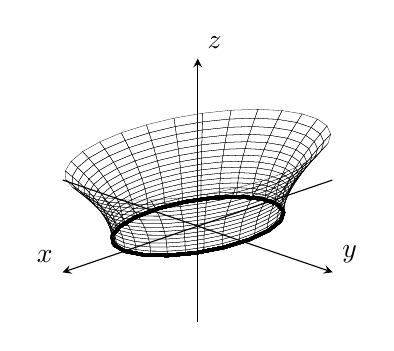
\begin{tikzpicture}
\begin{axis}[
  view={135}{20},
  axis lines=center,axis on top,
  ticks=none,set layers=default,axis equal,
  xlabel={$x$}, ylabel={$y$}, zlabel={$z$},
  xlabel style={anchor=south east},
  ylabel style={anchor=south west},
  zlabel style={anchor=south west},
  enlargelimits,
  tick align=inside,
  domain=0:2.00,
  samples=20,
  z buffer=sort,
]
  \def\a{0.8}
  \def\b{0.5}
  \def\c{0.5}
  \def\umax{1}

  \addplot3[
      mesh,
      samples=15,
      samples y=30,
      domain=0:\umax,
      domain y=0:360,
      draw=black,
      line width=0.1pt,
  ]
  (
      {\a*cosh(x)*cos(y)},
      {\b*cosh(x)*sin(y)},
      {\c*sinh(x)}
  );
  \addplot3[
      mesh,
      domain=0:360,
      samples=20,
      very thick,
      black
  ]
  (
    { \a*cos(x) },
    { \b*sin(x) },
    { 0 }
  );
\end{axis}
\end{tikzpicture}
\end{center}
Continued next lecture.
\end{document}
